\section{Thermodynamics}
The free energy\footnote{As we are in the grand canonical ensemble, this is the \emph{grand canonical} free energy, and not Helmholtz' free energy.}
is defined as
\begin{equation}
    \label{thermodynamic free energy}
    F = U - TS - \mu_I Q_I, \quad \dd F = - S \dd T - P \dd V - Q_I \dd \mu_I ,
\end{equation}
where $Q_I$ is the isospin charge, and $U$ is the energy.
As we have seen earlier, our system is homogenous.
This means that the free energy density is independent of volume, and thus $F = V \Ef$.
From 
\begin{equation}
    P = - \left(\diffp{F}{V}\right)_{T, \mu_I}
\end{equation}
We are interested in the pressure relative to $\mu_I$, 
\begin{equation}
    P(\mu_I) = -(\Ef(\mu_I) - \Ef(\mu_I = 0))
\end{equation}
This is illustrated in \autoref{fig:pressure}.
\begin{figure}[ht]
    \centering
    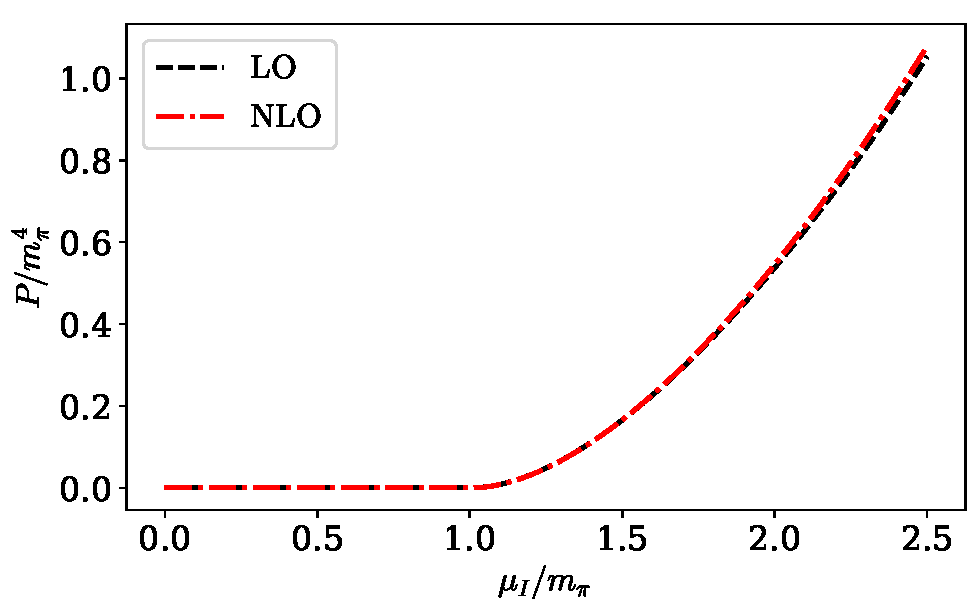
\includegraphics[width=0.8\textwidth]{figurer/numerics/pressure.pdf}
    \caption{The NLO and LO result for the pressure of the pions, as a function of $\mu_I$.}
    \label{fig:pressure}
\end{figure}
Likewise, the total isospin is proportional to volume, which means that the isospin density is
\begin{equation}
    n_I = \frac{Q_I}{V} = - \frac{1}{V} \left(\diffp{F}{\mu_I}\right)_{T, V}
    = - \diffp{\Ef}{\mu_I}.
\end{equation}
The isospin density, as a function of $\mu_I$, is shown in \autoref{fig:isospin_density}.
\begin{figure}
    \centering
    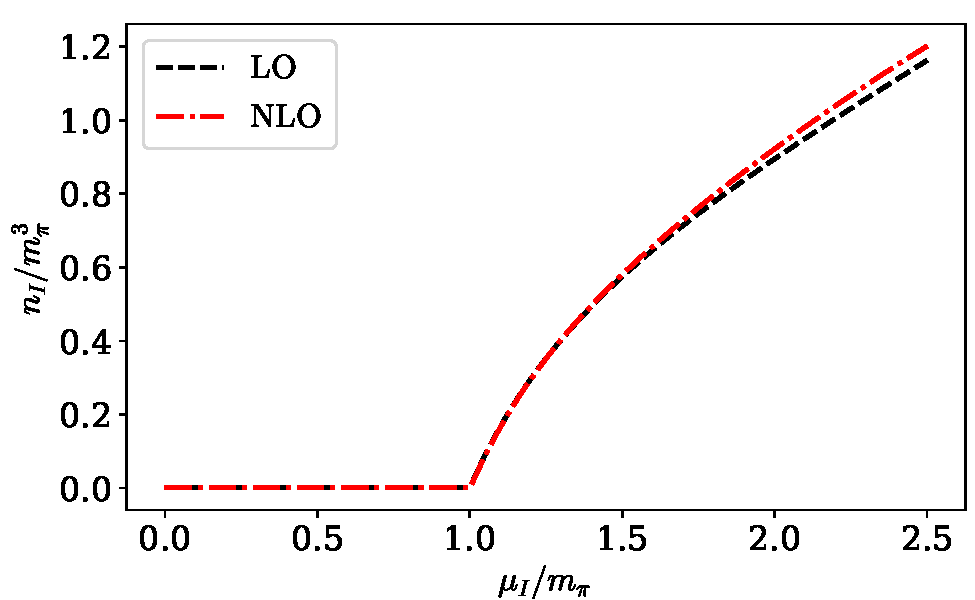
\includegraphics[width=0.8\textwidth]{figurer/numerics/isospin_density.pdf}
    \caption{The NLO and LO result for the isosopin densisty, as a function of $\mu_I$.}
    \label{fig:isospin_density}
\end{figure}
Finally, from \cref{thermodynamic free energy}, we get the energy density, $u = U/V$ is given by
\begin{equation}
    u(\mu_I) = -P(\mu_I) + \mu_I n_I(\mu_I).
\end{equation}
The isospin chemical potential $\mu_I$ parametrizes a line through the energy density-pressure plane, the relationship between the energy density and the pressure, which is shown in \autoref{fig:equation of state}.
This relationship has the form
\begin{equation}
    f(p, u) = 0,
\end{equation}
and is the equation of state of the pion system.


\begin{figure}[ht]
    \centering
    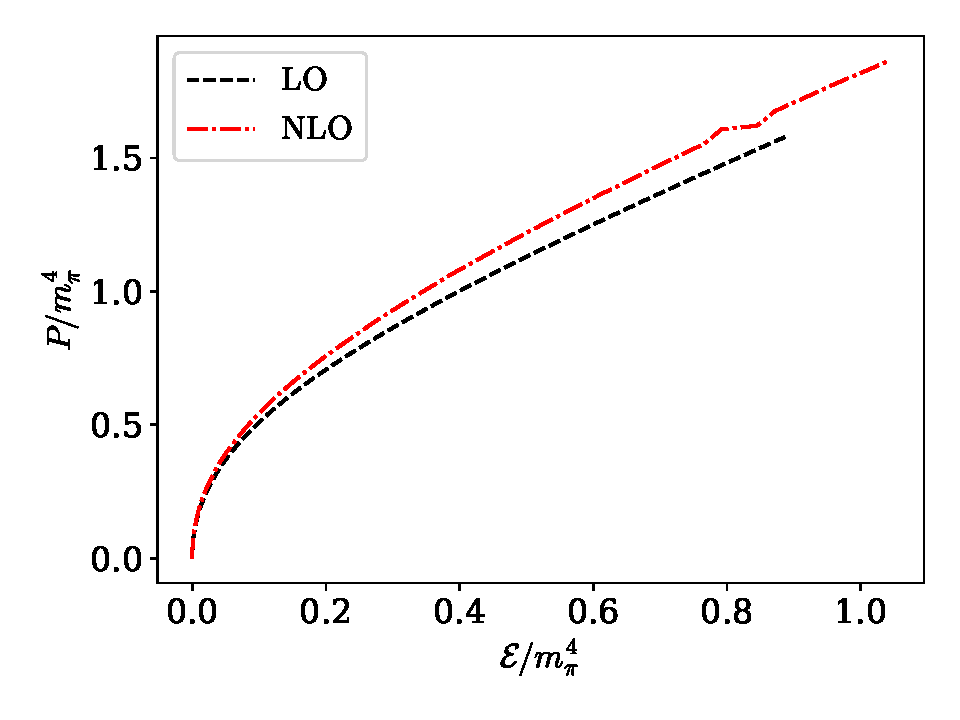
\includegraphics[width=0.8\textwidth]{figurer/numerics/energy_density.pdf}
    \caption{The equation of state of the pions.}
    \label{fig:equation of state}
\end{figure}
